\documentclass[12pt,a4paper,twoside,titlepage]{article}
\usepackage[utf8]{inputenc}
\usepackage[english]{babel}
\usepackage{utopia}
\usepackage[margin=1in]{geometry}
\usepackage[parfill]{parskip}
\usepackage{makeidx}
\usepackage{graphicx}
\usepackage[onehalfspacing]{setspace}
\usepackage{fancyhdr}
%\usepackage{lastpage}
\usepackage{hyperref}
\renewcommand{\sffamily}{phv}

\newcommand{\titleText}{DHCP Aufgabe Dokumentation}
\newcommand{\authorText}{Patrick Günthard}
\newcommand{\dateText}{\today}

\title{\titleText}
\author{\authorText}
\date{\dateText}

\pagestyle{fancy}
\fancyhf{}

\fancyhead[EL]{\titleText}
\fancyhead[OR]{\authorText}
\cfoot{\thepage}% \space von \pageref{LastPage}}

\begin{document}
	\maketitle
	\tableofcontents

        \section{Software Basis}

        \begin{tabular}{|l|l|}
          \hline
          \textbf{Server OS} & Debian GNU/Linux 8 Jessie \footnote{Im Text einfachheitshalber \textit{Debian-Server} oder \textit{Debian-System}}\\\hline
          \textbf{Client OS} & Windows Server 2012 R2 \footnote{Im Text einfachheitshalber \textit{Windows-Client} oder \textit{Windows-System}} \\\hline
          \textbf{DHCP Server} & isc-dhcp-server \\\hline
        \end{tabular}

        \section{Aufgabenstellung}

        Die grundlegende Aufgabe bestand darin, auf einer Linux-VM einen DHCP Server zu installieren und diesen dann mit einem Windows-Client (ebenfalls auf einer VM) zu testen.

        \section{Vorgehen}

        \subsection{Hürden}

        Es gab verschiedene Hürden beim aufsetzten des DHCP-Servers. Zu begin war nicht klar, welches package installiert werden sollte, da im Debian-Repository mehrere Implementierungen vorhanden sind. Ich entschied mich dann für den \textit{isc-dhcp-server} welcher weit verbreitet ist.
        
        \subsection{Lösungen}
        
        \section{Ergebnis \& Testprotokoll}

        \subsection{Ergebnis}

        \begin{figure}
          \center
          \label{fig:dynip}
          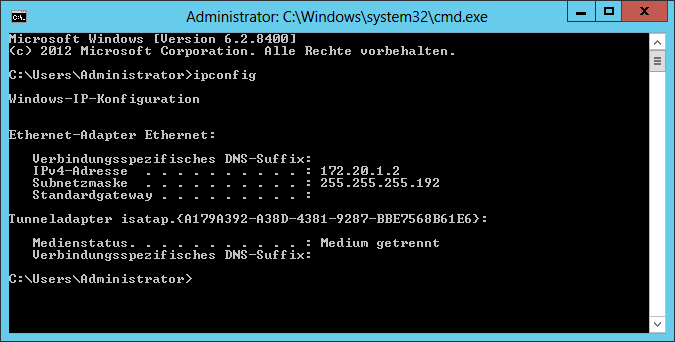
\includegraphics[width=8cm]{cmd_ipconfig_dynamic_ip}
          \caption{Dynamische IP}
        \end{figure}

        \begin{figure}
          \center
          \label{fig:webserver}
          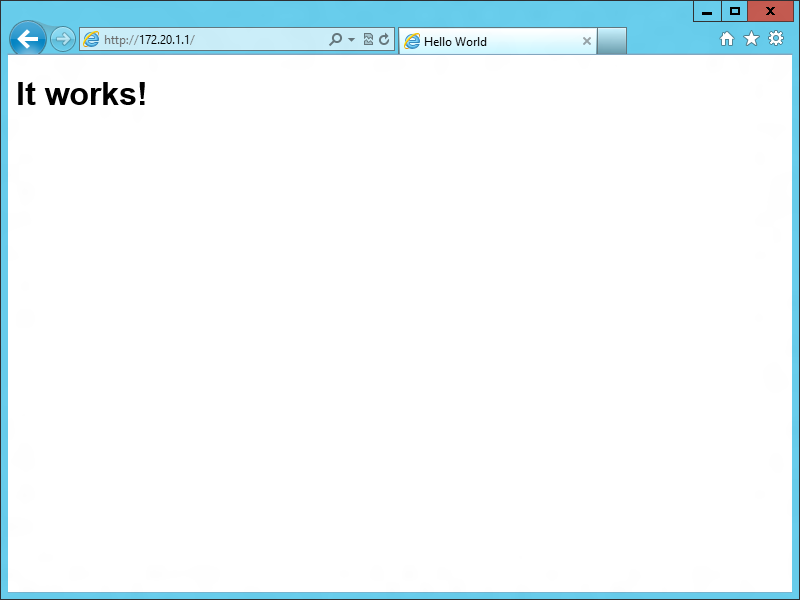
\includegraphics[width=8cm]{ie_web_example}
          \caption{Erfolgreicher Zugriff vom Windows Client auf den Webserver auf dem Debian Server}
        \end{figure}
        
        Das Endergebnis war eine Debian 8 Maschine mit funktionierendem DHCP Server. Das richtige funktionieren des Servers wurde mit einem Windows-Client getestet welcher beim starten automatisch eine IP des im Server definierten Bereiches übernahm \ref{fig:dynip}.

        Um zu testen ob auch eine Verbindung zwischen den beiden virtuellen Maschinen möglich ist, installierte ich auf dem Debian System ein Web-Server auf welchen ich auf dem Windows System erfolgreich zugreifen konnte \ref{fig:webserver}.

        \subsection{Testprotokoll}


        \begin{tabular}{|l|l|p{5cm}|}
          \hline
          \textbf{Aufgabe} & \textbf{Status \ref{statusref}} & \textbf{Kommentar} \\\hline
          Server OS Aufsetzen & & \\\hline
        \end{tabular}

        \label{statusref}
        \textit{E} = erreicht, \textit{T} = teilweise erreicht, \textit{N} = nicht erreicht 
        
        \section{Reflexion}
        
        
\end{document}
